\documentclass[twoside]{book}

% Packages required by doxygen
\usepackage{fixltx2e}
\usepackage{calc}
\usepackage{doxygen}
\usepackage[export]{adjustbox} % also loads graphicx
\usepackage{graphicx}
\usepackage[utf8]{inputenc}
\usepackage{makeidx}
\usepackage{multicol}
\usepackage{multirow}
\PassOptionsToPackage{warn}{textcomp}
\usepackage{textcomp}
\usepackage[nointegrals]{wasysym}
\usepackage[table]{xcolor}

% Font selection
\usepackage[T1]{fontenc}
\usepackage[scaled=.90]{helvet}
\usepackage{courier}
\usepackage{amssymb}
\usepackage{sectsty}
\renewcommand{\familydefault}{\sfdefault}
\allsectionsfont{%
  \fontseries{bc}\selectfont%
  \color{darkgray}%
}
\renewcommand{\DoxyLabelFont}{%
  \fontseries{bc}\selectfont%
  \color{darkgray}%
}
\newcommand{\+}{\discretionary{\mbox{\scriptsize$\hookleftarrow$}}{}{}}

% Page & text layout
\usepackage{geometry}
\geometry{%
  a4paper,%
  top=2.5cm,%
  bottom=2.5cm,%
  left=2.5cm,%
  right=2.5cm%
}
\tolerance=750
\hfuzz=15pt
\hbadness=750
\setlength{\emergencystretch}{15pt}
\setlength{\parindent}{0cm}
\setlength{\parskip}{3ex plus 2ex minus 2ex}
\makeatletter
\renewcommand{\paragraph}{%
  \@startsection{paragraph}{4}{0ex}{-1.0ex}{1.0ex}{%
    \normalfont\normalsize\bfseries\SS@parafont%
  }%
}
\renewcommand{\subparagraph}{%
  \@startsection{subparagraph}{5}{0ex}{-1.0ex}{1.0ex}{%
    \normalfont\normalsize\bfseries\SS@subparafont%
  }%
}
\makeatother

% Headers & footers
\usepackage{fancyhdr}
\pagestyle{fancyplain}
\fancyhead[LE]{\fancyplain{}{\bfseries\thepage}}
\fancyhead[CE]{\fancyplain{}{}}
\fancyhead[RE]{\fancyplain{}{\bfseries\leftmark}}
\fancyhead[LO]{\fancyplain{}{\bfseries\rightmark}}
\fancyhead[CO]{\fancyplain{}{}}
\fancyhead[RO]{\fancyplain{}{\bfseries\thepage}}
\fancyfoot[LE]{\fancyplain{}{}}
\fancyfoot[CE]{\fancyplain{}{}}
\fancyfoot[RE]{\fancyplain{}{\bfseries\scriptsize Generated by Doxygen }}
\fancyfoot[LO]{\fancyplain{}{\bfseries\scriptsize Generated by Doxygen }}
\fancyfoot[CO]{\fancyplain{}{}}
\fancyfoot[RO]{\fancyplain{}{}}
\renewcommand{\footrulewidth}{0.4pt}
\renewcommand{\chaptermark}[1]{%
  \markboth{#1}{}%
}
\renewcommand{\sectionmark}[1]{%
  \markright{\thesection\ #1}%
}

% Indices & bibliography
\usepackage{natbib}
\usepackage[titles]{tocloft}
\setcounter{tocdepth}{3}
\setcounter{secnumdepth}{5}
\makeindex

% Hyperlinks (required, but should be loaded last)
\usepackage{ifpdf}
\ifpdf
  \usepackage[pdftex,pagebackref=true]{hyperref}
\else
  \usepackage[ps2pdf,pagebackref=true]{hyperref}
\fi
\hypersetup{%
  colorlinks=true,%
  linkcolor=blue,%
  citecolor=blue,%
  unicode%
}

% Custom commands
\newcommand{\clearemptydoublepage}{%
  \newpage{\pagestyle{empty}\cleardoublepage}%
}

\usepackage{caption}
\captionsetup{labelsep=space,justification=centering,font={bf},singlelinecheck=off,skip=4pt,position=top}

%===== C O N T E N T S =====

\begin{document}

% Titlepage & ToC
\hypersetup{pageanchor=false,
             bookmarksnumbered=true,
             pdfencoding=unicode
            }
\pagenumbering{alph}
\begin{titlepage}
\vspace*{7cm}
\begin{center}%
{\Large My Project }\\
\vspace*{1cm}
{\large Generated by Doxygen 1.8.13}\\
\end{center}
\end{titlepage}
\clearemptydoublepage
\pagenumbering{roman}
\tableofcontents
\clearemptydoublepage
\pagenumbering{arabic}
\hypersetup{pageanchor=true}

%--- Begin generated contents ---
\chapter{Namespace Index}
\section{Packages}
Here are the packages with brief descriptions (if available)\+:\begin{DoxyCompactList}
\item\contentsline{section}{\hyperlink{namespace_wpf_application10}{Wpf\+Application10} }{\pageref{namespace_wpf_application10}}{}
\end{DoxyCompactList}

\chapter{Hierarchical Index}
\section{Class Hierarchy}
This inheritance list is sorted roughly, but not completely, alphabetically\+:\begin{DoxyCompactList}
\item Application\begin{DoxyCompactList}
\item \contentsline{section}{Wpf\+Application10.\+App}{\pageref{class_wpf_application10_1_1_app}}{}
\end{DoxyCompactList}
\item Button\begin{DoxyCompactList}
\item \contentsline{section}{Wpf\+Application10.\+Cella}{\pageref{class_wpf_application10_1_1_cella}}{}
\end{DoxyCompactList}
\item Canvas\begin{DoxyCompactList}
\item \contentsline{section}{Wpf\+Application10.\+Campo}{\pageref{class_wpf_application10_1_1_campo}}{}
\end{DoxyCompactList}
\item Window\begin{DoxyCompactList}
\item \contentsline{section}{Wpf\+Application10.\+Main\+Window}{\pageref{class_wpf_application10_1_1_main_window}}{}
\end{DoxyCompactList}
\end{DoxyCompactList}

\chapter{Class Index}
\section{Class List}
Here are the classes, structs, unions and interfaces with brief descriptions\+:\begin{DoxyCompactList}
\item\contentsline{section}{\hyperlink{class_wpf_application10_1_1_app}{Wpf\+Application10.\+App} \\*Logica di interazione per App.\+xaml }{\pageref{class_wpf_application10_1_1_app}}{}
\item\contentsline{section}{\hyperlink{class_wpf_application10_1_1_campo}{Wpf\+Application10.\+Campo} \\*Aggregato di Celle simula il campo di gioco }{\pageref{class_wpf_application10_1_1_campo}}{}
\item\contentsline{section}{\hyperlink{class_wpf_application10_1_1_cella}{Wpf\+Application10.\+Cella} \\*Classe del bottono elementare del campo minato }{\pageref{class_wpf_application10_1_1_cella}}{}
\item\contentsline{section}{\hyperlink{class_wpf_application10_1_1_main_window}{Wpf\+Application10.\+Main\+Window} }{\pageref{class_wpf_application10_1_1_main_window}}{}
\end{DoxyCompactList}

\chapter{Namespace Documentation}
\hypertarget{namespace_wpf_application10}{}\section{Wpf\+Application10 Namespace Reference}
\label{namespace_wpf_application10}\index{Wpf\+Application10@{Wpf\+Application10}}
\subsection*{Classes}
\begin{DoxyCompactItemize}
\item 
class \hyperlink{class_wpf_application10_1_1_app}{App}
\begin{DoxyCompactList}\small\item\em Logica di interazione per App.\+xaml \end{DoxyCompactList}\item 
class \hyperlink{class_wpf_application10_1_1_campo}{Campo}
\begin{DoxyCompactList}\small\item\em Aggregato di Celle simula il campo di gioco. \end{DoxyCompactList}\item 
class \hyperlink{class_wpf_application10_1_1_cella}{Cella}
\begin{DoxyCompactList}\small\item\em classe del bottono elementare del campo minato \end{DoxyCompactList}\item 
class \hyperlink{class_wpf_application10_1_1_main_window}{Main\+Window}
\end{DoxyCompactItemize}

\chapter{Class Documentation}
\hypertarget{class_wpf_application10_1_1_app}{}\section{Wpf\+Application10.\+App Class Reference}
\label{class_wpf_application10_1_1_app}\index{Wpf\+Application10.\+App@{Wpf\+Application10.\+App}}


Logica di interazione per App.\+xaml  


Inheritance diagram for Wpf\+Application10.\+App\+:\begin{figure}[H]
\begin{center}
\leavevmode
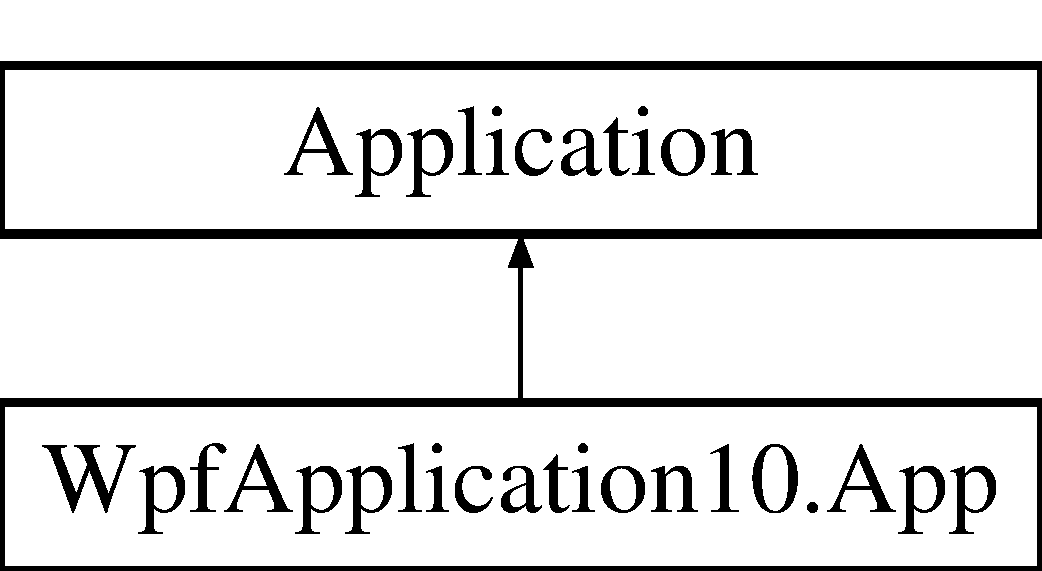
\includegraphics[height=2.000000cm]{class_wpf_application10_1_1_app}
\end{center}
\end{figure}


\subsection{Detailed Description}
Logica di interazione per App.\+xaml 



The documentation for this class was generated from the following file\+:\begin{DoxyCompactItemize}
\item 
App.\+xaml.\+cs\end{DoxyCompactItemize}

\hypertarget{class_wpf_application10_1_1_campo}{}\section{Wpf\+Application10.\+Campo Class Reference}
\label{class_wpf_application10_1_1_campo}\index{Wpf\+Application10.\+Campo@{Wpf\+Application10.\+Campo}}


Aggregato di Celle simula il campo di gioco.  


Inheritance diagram for Wpf\+Application10.\+Campo\+:\begin{figure}[H]
\begin{center}
\leavevmode
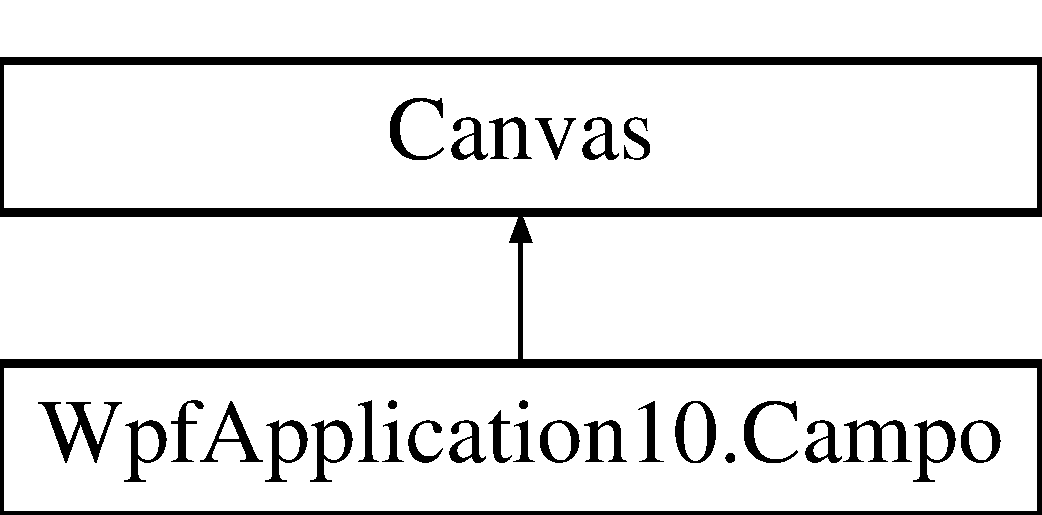
\includegraphics[height=2.000000cm]{class_wpf_application10_1_1_campo}
\end{center}
\end{figure}
\subsection*{Public Member Functions}
\begin{DoxyCompactItemize}
\item 
\mbox{\Hypertarget{class_wpf_application10_1_1_campo_aef7860620b7283130d210748331a0a80}\label{class_wpf_application10_1_1_campo_aef7860620b7283130d210748331a0a80}} 
\hyperlink{class_wpf_application10_1_1_campo_aef7860620b7283130d210748331a0a80}{Campo} (int grandezza)
\begin{DoxyCompactList}\small\item\em Prende in ingresso la grandezza della matrice. \end{DoxyCompactList}\item 
\mbox{\Hypertarget{class_wpf_application10_1_1_campo_a626ff5f098dc2c30a4907664671c74ae}\label{class_wpf_application10_1_1_campo_a626ff5f098dc2c30a4907664671c74ae}} 
void {\bfseries refresh} ()
\item 
\mbox{\Hypertarget{class_wpf_application10_1_1_campo_ac5b29a3446d94cd6fd70229f126a63be}\label{class_wpf_application10_1_1_campo_ac5b29a3446d94cd6fd70229f126a63be}} 
void {\bfseries genera\+Bomba} (int n\+Bombe, Random rnd)
\item 
void \hyperlink{class_wpf_application10_1_1_campo_ab70e4d4a95b9d7660c361c8ab2b103fc}{calcola\+Valore} ()
\begin{DoxyCompactList}\small\item\em Una volta assegnata le bombe calcola i valori delle caselle cirdostanti. \end{DoxyCompactList}\item 
\mbox{\Hypertarget{class_wpf_application10_1_1_campo_a1665e095674df35485694fd7aafd0475}\label{class_wpf_application10_1_1_campo_a1665e095674df35485694fd7aafd0475}} 
void {\bfseries controllo} (int x\+\_\+, int y\+\_\+)
\end{DoxyCompactItemize}
\subsection*{Public Attributes}
\begin{DoxyCompactItemize}
\item 
\mbox{\Hypertarget{class_wpf_application10_1_1_campo_a01b0b1aa98788bb40190d216cd91e89f}\label{class_wpf_application10_1_1_campo_a01b0b1aa98788bb40190d216cd91e89f}} 
\hyperlink{class_wpf_application10_1_1_cella}{Cella} \mbox{[},\mbox{]} \hyperlink{class_wpf_application10_1_1_campo_a01b0b1aa98788bb40190d216cd91e89f}{matrice}
\begin{DoxyCompactList}\small\item\em Matrice di celle. \end{DoxyCompactList}\item 
\mbox{\Hypertarget{class_wpf_application10_1_1_campo_a2b85b75097ce72b3d29aacca2cb3a1f6}\label{class_wpf_application10_1_1_campo_a2b85b75097ce72b3d29aacca2cb3a1f6}} 
int {\bfseries gran}
\end{DoxyCompactItemize}


\subsection{Detailed Description}
Aggregato di Celle simula il campo di gioco. 

\subsection{Member Function Documentation}
\mbox{\Hypertarget{class_wpf_application10_1_1_campo_ab70e4d4a95b9d7660c361c8ab2b103fc}\label{class_wpf_application10_1_1_campo_ab70e4d4a95b9d7660c361c8ab2b103fc}} 
\index{Wpf\+Application10\+::\+Campo@{Wpf\+Application10\+::\+Campo}!calcola\+Valore@{calcola\+Valore}}
\index{calcola\+Valore@{calcola\+Valore}!Wpf\+Application10\+::\+Campo@{Wpf\+Application10\+::\+Campo}}
\subsubsection{\texorpdfstring{calcola\+Valore()}{calcolaValore()}}
{\footnotesize\ttfamily Wpf\+Application10.\+Campo.\+calcola\+Valore (\begin{DoxyParamCaption}{ }\end{DoxyParamCaption})}



Una volta assegnata le bombe calcola i valori delle caselle cirdostanti. 

\begin{DoxyNote}{Note}
Ciclo su tutte le caselle

verifico che la casella non sia una bomba

controllo le caselle adiacenti

controllo l\textquotesingle{}indice della matrice 
\end{DoxyNote}


The documentation for this class was generated from the following file\+:\begin{DoxyCompactItemize}
\item 
Campo.\+cs\end{DoxyCompactItemize}

\hypertarget{class_wpf_application10_1_1_cella}{}\section{Wpf\+Application10.\+Cella Class Reference}
\label{class_wpf_application10_1_1_cella}\index{Wpf\+Application10.\+Cella@{Wpf\+Application10.\+Cella}}


classe del bottono elementare del campo minato  


Inheritance diagram for Wpf\+Application10.\+Cella\+:\begin{figure}[H]
\begin{center}
\leavevmode
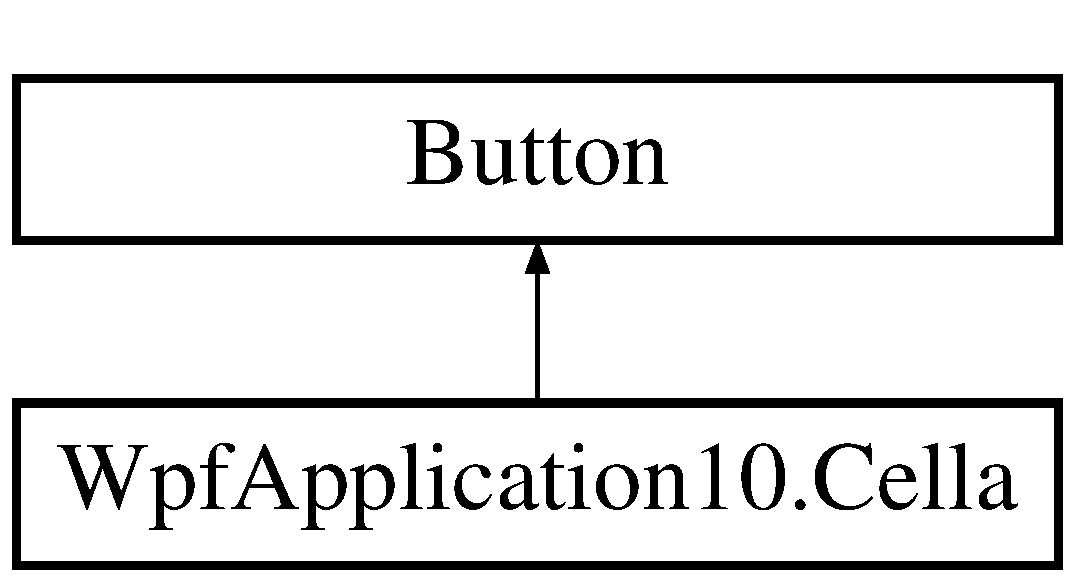
\includegraphics[height=2.000000cm]{class_wpf_application10_1_1_cella}
\end{center}
\end{figure}
\subsection*{Public Member Functions}
\begin{DoxyCompactItemize}
\item 
\mbox{\Hypertarget{class_wpf_application10_1_1_cella_a862cd54e4059b6b1d5f01d530b56b54d}\label{class_wpf_application10_1_1_cella_a862cd54e4059b6b1d5f01d530b56b54d}} 
\hyperlink{class_wpf_application10_1_1_cella_a862cd54e4059b6b1d5f01d530b56b54d}{Cella} (int \hyperlink{class_wpf_application10_1_1_cella_a6f0eb1102ff02ab27e3767c5c5852598}{x}, int \hyperlink{class_wpf_application10_1_1_cella_a2b648fcacbaf4ec37274633409f00e5e}{y})
\begin{DoxyCompactList}\small\item\em Costruttore imposta il valore della cella a 0 e le dimensioni del bottone a 50\+:50. \end{DoxyCompactList}\item 
\mbox{\Hypertarget{class_wpf_application10_1_1_cella_adc88e8ad6e5b9b34f5915e338c7a9fd7}\label{class_wpf_application10_1_1_cella_adc88e8ad6e5b9b34f5915e338c7a9fd7}} 
void {\bfseries Mostra\+Valore} ()
\end{DoxyCompactItemize}
\subsection*{Properties}
\begin{DoxyCompactItemize}
\item 
\mbox{\Hypertarget{class_wpf_application10_1_1_cella_a2e829f534fc0c3bbcdcba638db628940}\label{class_wpf_application10_1_1_cella_a2e829f534fc0c3bbcdcba638db628940}} 
int {\bfseries valore}\hspace{0.3cm}{\ttfamily  \mbox{[}get, set\mbox{]}}
\item 
\mbox{\Hypertarget{class_wpf_application10_1_1_cella_a6f0eb1102ff02ab27e3767c5c5852598}\label{class_wpf_application10_1_1_cella_a6f0eb1102ff02ab27e3767c5c5852598}} 
int \hyperlink{class_wpf_application10_1_1_cella_a6f0eb1102ff02ab27e3767c5c5852598}{x}\hspace{0.3cm}{\ttfamily  \mbox{[}get, set\mbox{]}}
\begin{DoxyCompactList}\small\item\em variabile che indica la posizione x nella matrice \end{DoxyCompactList}\item 
\mbox{\Hypertarget{class_wpf_application10_1_1_cella_a2b648fcacbaf4ec37274633409f00e5e}\label{class_wpf_application10_1_1_cella_a2b648fcacbaf4ec37274633409f00e5e}} 
int \hyperlink{class_wpf_application10_1_1_cella_a2b648fcacbaf4ec37274633409f00e5e}{y}\hspace{0.3cm}{\ttfamily  \mbox{[}get, set\mbox{]}}
\begin{DoxyCompactList}\small\item\em variabile che indica la posizione y nella matrice \end{DoxyCompactList}\end{DoxyCompactItemize}


\subsection{Detailed Description}
classe del bottono elementare del campo minato 

The documentation for this class was generated from the following file\+:\begin{DoxyCompactItemize}
\item 
Cella.\+cs\end{DoxyCompactItemize}

\hypertarget{class_wpf_application10_1_1_main_window}{}\section{Wpf\+Application10.\+Main\+Window Class Reference}
\label{class_wpf_application10_1_1_main_window}\index{Wpf\+Application10.\+Main\+Window@{Wpf\+Application10.\+Main\+Window}}
Inheritance diagram for Wpf\+Application10.\+Main\+Window\+:\begin{figure}[H]
\begin{center}
\leavevmode
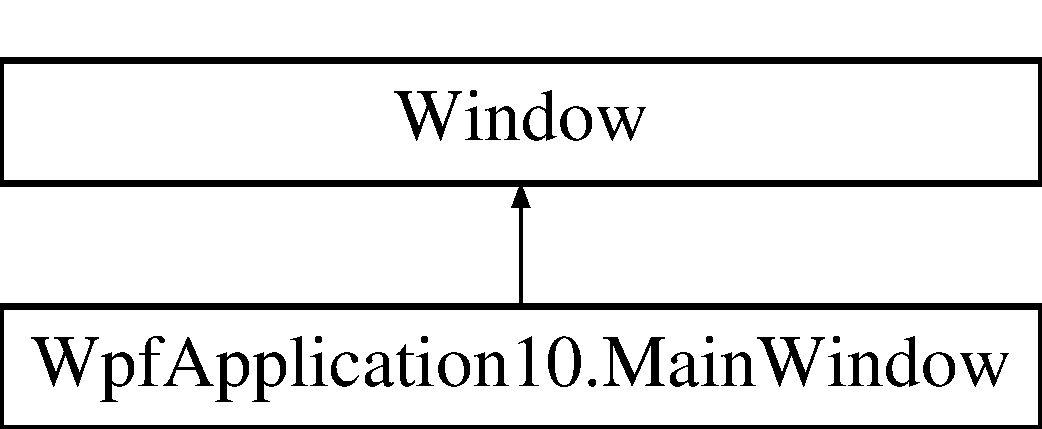
\includegraphics[height=2.000000cm]{class_wpf_application10_1_1_main_window}
\end{center}
\end{figure}
\subsection*{Public Attributes}
\begin{DoxyCompactItemize}
\item 
\mbox{\Hypertarget{class_wpf_application10_1_1_main_window_a9cbba2eb3afe7eb26c5b89dfd9ed8e8b}\label{class_wpf_application10_1_1_main_window_a9cbba2eb3afe7eb26c5b89dfd9ed8e8b}} 
\hyperlink{class_wpf_application10_1_1_cella}{Cella} {\bfseries prova} = new \hyperlink{class_wpf_application10_1_1_cella}{Cella}(3,3)
\item 
\mbox{\Hypertarget{class_wpf_application10_1_1_main_window_a974cb0754fff931a7d2ae34f096eceed}\label{class_wpf_application10_1_1_main_window_a974cb0754fff931a7d2ae34f096eceed}} 
Random {\bfseries rnd} = new Random()
\item 
\mbox{\Hypertarget{class_wpf_application10_1_1_main_window_a1767b2d31ae24ab8c180f833472a7a79}\label{class_wpf_application10_1_1_main_window_a1767b2d31ae24ab8c180f833472a7a79}} 
\hyperlink{class_wpf_application10_1_1_campo}{Campo} {\bfseries c} = new \hyperlink{class_wpf_application10_1_1_campo}{Campo}(3)
\end{DoxyCompactItemize}


The documentation for this class was generated from the following file\+:\begin{DoxyCompactItemize}
\item 
Main\+Window.\+xaml.\+cs\end{DoxyCompactItemize}

%--- End generated contents ---

% Index
\backmatter
\newpage
\phantomsection
\clearemptydoublepage
\addcontentsline{toc}{chapter}{Index}
\printindex

\end{document}
